% #############################################################################
% This is Chapter 1
% !TEX root = ../main.tex
% #############################################################################
% Change the Name of the Chapter i the following line
\fancychapter{Introduction}
\cleardoublepage
% The following line allows to ref this chapter
\label{chap:intro}
	
	The act of making things as perfect, functional, or effective as possible is a process known as optimization~\cite{MerriamWebster2017OptimizationDefinition}. Intuitively, through optimization one aims to improve different quantitative measurable aspects. However, sometimes, instead of trying to achieve perfection, finding a better outcome or a near-optimal one suffices. %Although usually striving to fully optimize, i.e., to obtain \textit{perfection}, in some cases, finding a better outcome or a near-optimal one suffices.
	
	Optimization has a paramount impact in the fields of economy, science, and engineering, among others. As a case in point, optimization yields great potential to the architecture field, as it directly impacts the building industry: optimization enables the reduction of the economic and ecological footprint of the building sector through the finding of more efficient building variants, prior to their construction. 
	
	Modern architecture has grown to incorporate economic and environmental concerns into its building design practices by introducing standardized building regulations and energy certificates. These concerns led to the creation of new design approaches, such as \ac{PBD} which seeks for more efficient design solutions by considering the design's performance, possibly measured by using computational tools~\cite{Oxman2006PBD}.
	
	One example of the \ac{PBD} approach is the City Hall in London, shown in \cref{fig:cityhalllondon}. The building was designed to achieve optimum energy performance by minimizing the surface area exposed to direct sunlight, thus originating its spherical-like form. The application of energy-saving techniques, such as leaning the building outwards so that the floorplates provide shading to the floors below, or the use of groundwater from the water table to supply the building's cooling system, reduced the need for additional cooling devices and, consequently, enabled the energy consumed by the building to be 75\% lower than the energy consumed by typical air-conditioned office buildings \cite{Malkawi2005}.
	% , the use of groundwater from the water table to supply the building's cooling system, and the use of photovoltaic panels on the top of the building to maximize direct sunlight,
	\begin{figure}[htbp]
		\centering
		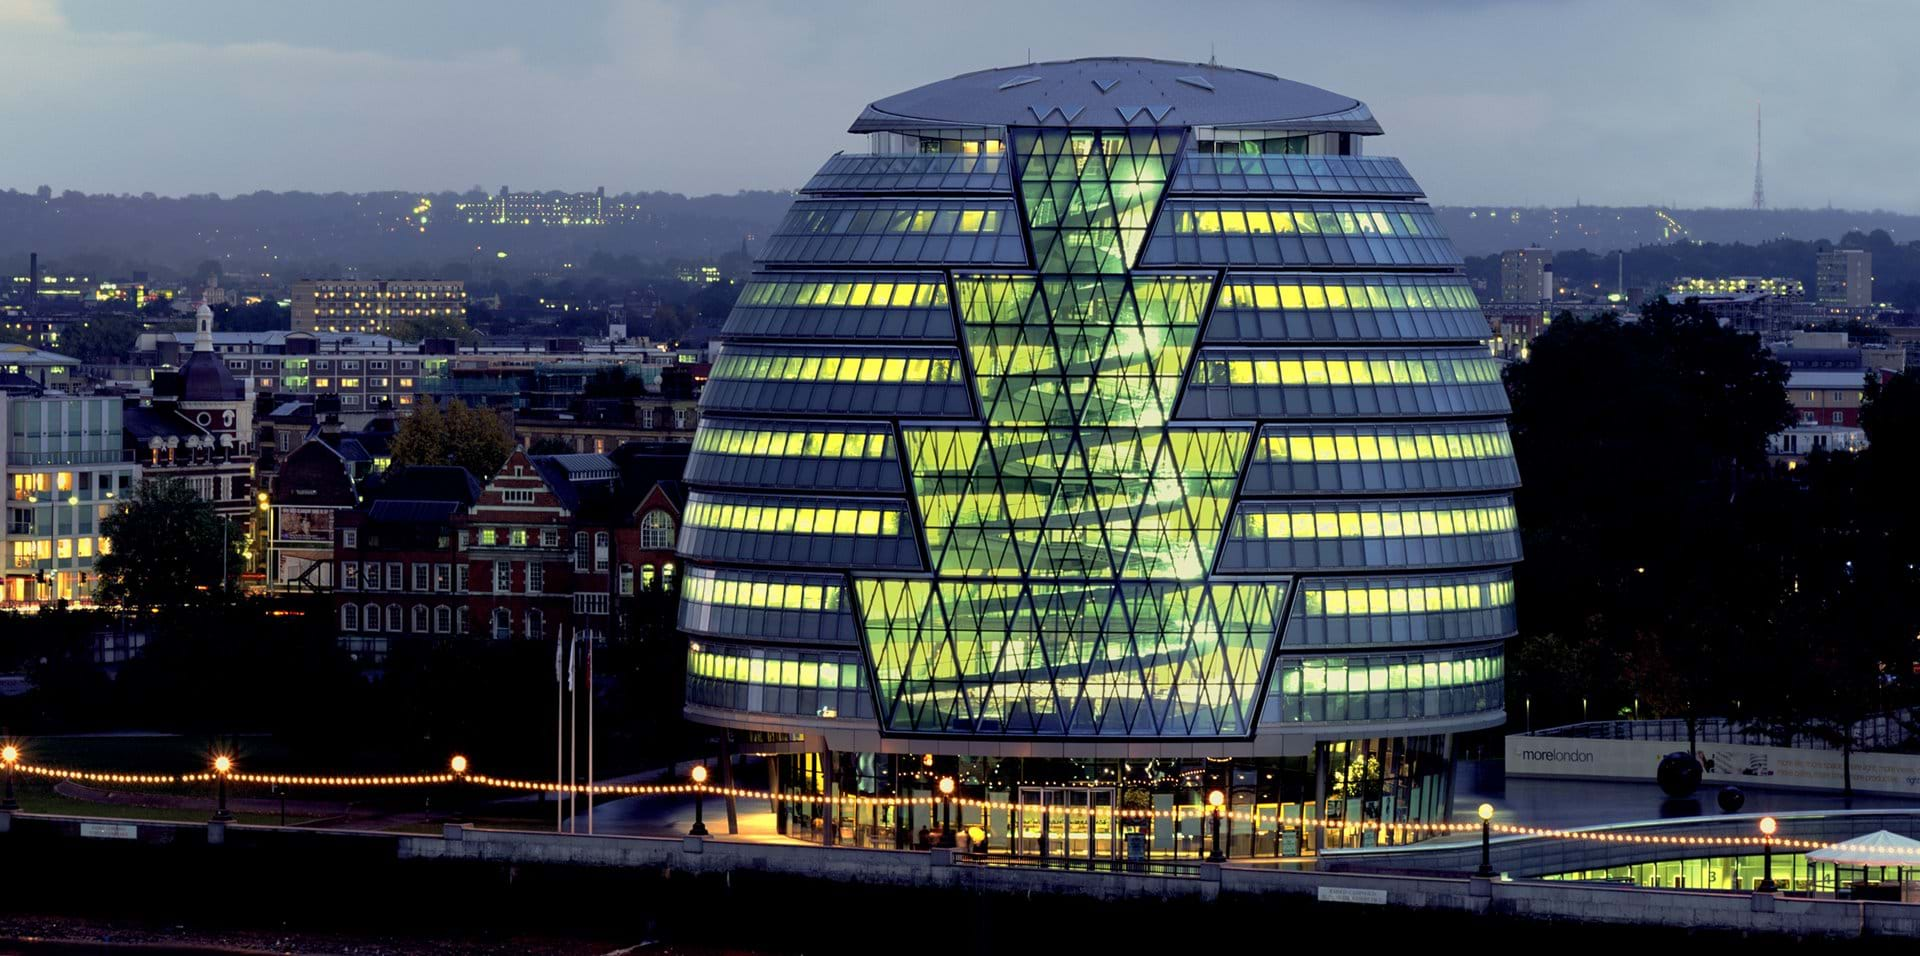
\includegraphics[width=\textwidth]{./Images/Introduction/cityhalllondon.jpg}
		\caption[City Hall in London, designed by Foster and Partners]{City Hall in London, designed by Foster+Partners. Image retrieved from \cite{londoncityhall}.}
		\label{fig:cityhalllondon}
	\end{figure}

	Notwithstanding the benefits attained with \ac{PBD}, to achieve the most performant designs regarding a certain aspect (e.g., lighting, structural, cost), the evaluation of multiple design variants is required. However, even a single evaluation may take up to several seconds, minutes, hours, or days to complete. This is particularly problematic in building design, which frequently requires the evaluation of multiple conflicting aspects, e.g., maximum lighting and thermal comfort, and minimum energy consumption. Adding to this complexity, \ac{PBD} approaches often require architects to perform several manual and time-consuming interventions in order to guarantee that the results meet the standard requirements. The time complexity and the constant need for manual interventions limit the number of design variations evaluated during a \ac{PBD} approach and, consequently, lead to designs that are far from being optimal.  
	
	Given the relevance of \ac{PBD} to the world's sustainability and economy, this dissertation attempts to automate the \ac{PBD} process and, consequently, maximize its potential to the architectural practice. To this end, we address optimization algorithms especially targeted to solve problems involving expensive evaluation functions and we develop an optimization framework that supports their application within the architectural practice to create optimized designs. To better understand which algorithms to use and how to tackle \ac{PBD}'s time limitations, we must consider the two main stages of \ac{PBD} processes: design and analysis. While in the former, the architect creates a design, in the latter, the architect evaluates the design's performance, possibly by using computational analysis tools. To deal with the exploration of several design alternatives, this dissertation proposes a framework capable of generating and evaluating design variants, using the results of each evaluation to search for more efficient designs.
	
	The following sections of this chapter describe the evolution of the optimization practice in architecture, evidencing the limitations of different design processes and the foundations for the creation of an automatic optimization framework for architecture. Finally, we end by highlighting the dissertation's research goals and its structure.

%% #############################################################################
\section{From Design to Optimized Design}
	
	In architecture, optimization has been gaining relevance for the past few years, especially due to the impact of building construction and maintenance in the world's economy and environment~\cite{Attia2013, Shi2016}. For this reason, designers are now shifting their design methods to incorporate \ac{PBD}, where buildings are optimized to achieve the best possible values regarding different characteristics of their design, such as thermal comfort, energy consumption, lighting comfort, structural behavior, cost, among others.

	This has only been possible due to the technological improvements in the architectural practice over the last few decades. The adoption of digital modeling tools allowed for a more accurate and efficient design of highly complex buildings. These tools enabled the shift from traditional paper-based approaches to more computerized ones, such as \ac{CAD} and \ac{BIM} approaches, where changes to designs are facilitated, not requiring architects to manually erase and redraw parts of the original design \cite{Ferreira2015GD}. \Cref{fig:traditionaldesign} illustrates a general view of such computational design process, as well as an example of a 3D modeling tool. The architect interacts directly with the modeling tools to incrementally develop his design ideas.
	
\begin{figure*}[htbp]
\centering
\subfigure[]{%
\label{fig:traditionaldesign-a}%

\includegraphics[width=0.38\textwidth]{./Images/Introduction/TraditionalArchitecturalDesign.png}}%
\hfill
\subfigure[]{%
\label{fig:traditionaldesign-b}%
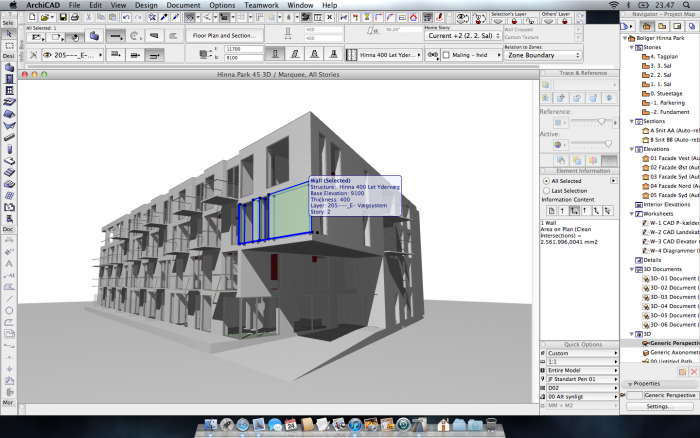
\includegraphics[width=0.48\textwidth]{./Images/Introduction/Example3DModellingTool_1.png}}%

\caption[General view of a traditional design approach]{(a) Simplification of a computational design workflow (b) An example of a building design in a 3D modeling tool. Image retrieved from \cite{3DMODELTOOL}.}
\label{fig:traditionaldesign}
\end{figure*}

Shortly after, the development of computer-based simulation tools enabled designers to simulate the behavior of their designs regarding specific criteria, i.e., to get a measurement of the designs' performance \cite{Malkawi2005}. Through this process, known as \ac{BPS}, designers can validate whether their design's performance satisfies the efficiency requirements and, ultimately, optimize the design by iteratively remodeling the geometry in order to obtain variations, assessing their performance, and selecting the better ones. Albeit still being very primitive, architects now have the elementary mechanisms required for optimizing their building's designs, which spurs a new \ac{PBD} approach: \ac{BPO}.

% #############################################################################
\subsection{Building Performance Optimization}

	\ac{BPO}, a simulation-based optimization approach, treats the results produced by simulation tools as the functions to optimize. Although suffering from some degree of imprecision and inaccuracy, these simulations make it possible to estimate the performance of complex designs. Particularly, these estimates are beneficial in designs for which analytical solutions are difficult or even impossible to derive \cite{Kolda2003}. In these cases, the objective function, i.e., the function to optimize, is derived from the simulations' results. The domain of these functions corresponds to the range of acceptable designs,  which is specified by the architect.

	A known drawback of simulation-based approaches is the time required to achieve reasonable results for complex systems~\cite{Law1991}, which is associated with different aspects of the problem, namely: (1) its \textbf{domain} which, depending on the nature of the problem, might use different methodologies to produce the corresponding estimates (e.g., thermal \textit{versus} structural); (2) its \textbf{intrinsic structure} that, depending on the attributes and relations of the system, might lead either to simpler or to more complicated computations (e.g., skyscraper \textit{versus} a small house); and (3) its \textbf{analytical model}, i.e., a model containing the essential properties of the system we are trying to simulate and that will be used as input to the simulation tool. Generally, the domain and structure do not change for the same problem, however there are numerous ways to produce multiple analytical models. Depending on the level of detail of the analytical model, both the computational time and results of the simulation might change. 

	In architecture, the production of analytical models is a complex and tiresome task. On the one hand, it is often necessary to produce multiple analytical models of the same design because of the different simulation tools' specificities, i.e., each simulation tool requires its own specialized model of the same design. On the other hand, simulation is often a time-consuming process due to the amount of computation that is required.

% Motivation for other design alternatives
	Finally, a \ac{BPO} methodology requires the evaluation of different design variations, which, if done manually, implies spending a large amount of time with the application of changes to the design. Despite the flexibility provided by \ac{CAD} and \ac{BIM} tools, architects often face difficulties when modeling complex geometry. As a result, the whole optimization process becomes unviable.
	
% #############################################################################
\subsection{Algorithmic Design}
\label{ssec:ad}
% Introduction to AD, way of overcoming limitations of manual approaches
	A design approach capable of creating forms through algorithms is crucial for overcoming the aforementioned limitations. An example of such an approach is \ac{AD}~\cite{Branco2017AD} and \cref{fig:algorithmicdesign} illustrates a simplified scheme of its application in the architectural design workflow. In this approach, the architect develops an algorithmic description of the intended design, that, when executed, generates the corresponding 3D model in an architectural modeling tool, such as a \ac{CAD} or \ac{BIM} tool. Algorithmic approaches are inherently parametric, enabling the generation of different variations of the same design by simply modifying the parameters' values~\cite{Leitao2014GD}. 
	
\begin{figure}[htbp]
\centering

\includegraphics[width=0.70\textwidth]{./Images/Introduction/AlgorithmicArchitecturalDesign.png}
\caption[General view of the Algorithmic Design approach]{Algorithmic Design workflow.}
\label{fig:algorithmicdesign}
\end{figure}
	
	As an example, consider the algorithmic design of Astana's National Library by Bjarke Ingels Group (BIG) architects, illustrated in~\cref{fig:astana-a}. Since the library's shape resembles a \textit{möbius} strip, its algorithmic description is defined in terms of several parameters, amongst which the radius and the number of turns of the strip. Thus, by invoking the algorithm with different values for these parameters, the architect can easily generate different variations of the building. \Cref{fig:astana-b,fig:astana-c} illustrate two design variations, where the radius and number of turns are increased, respectively.
	
\begin{figure*}[htbp]
\centering
\subfigure[]{%
\label{fig:astana-a}%
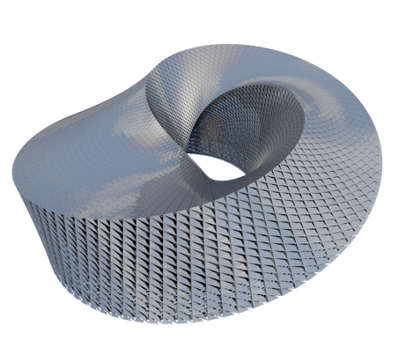
\includegraphics[width=0.32\textwidth]{./Images/Astana/Astana1.png}}%
\hfill
\subfigure[]{%
\label{fig:astana-b}%
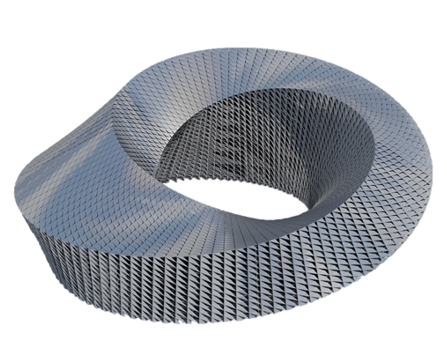
\includegraphics[width=0.33\textwidth]{./Images/Astana/Astana2.png}}%
\hfill
\subfigure[]{%
\label{fig:astana-c}%
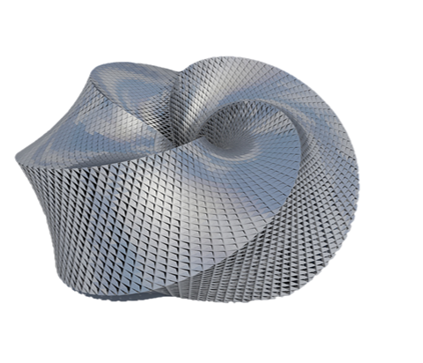
\includegraphics[width=0.33\textwidth]{./Images/Astana/Astana3.png}}%

\caption[Design variations of the Astana's National Library]{Design variations of the Astana National Library: (a) Original; (b) Larger diameter; (c) Two \textit{möbius} turns. Images adapted from \cite{Branco2017AD}.}
\label{fig:astana}
\end{figure*}

% Advantages over Manual approaches & Disadvantages
Only recently has the algorithmic paradigm begun to settle in the architectural practice. The need for programming knowledge is often an obstacle to the adoption of this paradigm, since it requires a large initial investment for architects to learn such techniques. Despite these investments, the benefits arising from the use of \ac{AD} approaches surpass those of directly using \ac{CAD} or \ac{BIM} tools to design complex buildings. Particularly, the initial investment is quickly recovered when the need for the incorporation of changes arises or when it becomes necessary to experiment different design variations. This is especially important when facing design processes that are characterized by constant changes to the project's constraints and requirements. In these scenarios, a manual-based approach requires constant manual changes to the model, thus incurring a dreadful and tiresome process, whereas an algorithmic approach enables the effortless generation of a broader range of design solutions, as well as the easy modification of the models to comply with new requirements. As a result, using \ac{AD}, architects are able to explore larger regions of the solution space, i.e., the set of possible design solutions, as well as innovative solutions that were not previously considered due to the time and effort required~\cite{Leitao2014GD}.

Another benefit of the \ac{AD} approach is the ease of maintenance of the models involved in building design. In fact, since \ac{AD} usually requires a single algorithmic description of the design, i.e., the algorithmic model, it is easier to maintain in scenarios where changes are frequent. On the other hand, manual-based-approaches often involve the creation and maintenance of multiple models of the same design (e.g., analytical models, 3D models), which quickly becomes hard and tiresome.

% Conclusion
The emergence of \ac{AD} was crucial for the automation of optimization processes by enabling the automatic generation of multiple design solutions. However, the optimization of these designs requires the creation of the corresponding analytical models, which can be very different from the 3D models originally produced by the \ac{AD} tool. Therefore, to evaluate the models produced by the \ac{AD} tool, the architect must manually generate the analytical model for each variation. Particularly, when dealing with complex buildings, this task requires a large amount of time and effort, which makes the optimization process almost impracticable.

% #############################################################################
\subsection{Algorithmic Analysis}
\label{ssec:aa}

% Motivação p/ passar de AD p/ AA.
Faster and broader design space exploration prompted the creation of increasingly complex building designs, which became less predictable with respect to different aspects~\cite{Branco2017AD}, such as thermal, lighting, acoustics, among others. Moreover, the recent focus on efficient and sustainable buildings led to the demand for buildings that, not only are well-designed, but also exhibit good performance in those aspects.
	
% Motivar necessidade de ferramentas de tradução de modelos 
Nowadays, most of the available simulation-based analysis tools are single-domain, each one evaluating the metrics that are specific of the domain~\cite{Malkawi2005}, i.e., while a lighting analysis tool measures daylight and glare coefficients, an energy simulation tool measures the coefficients related to energy consumption, ventilation, and air conditioning systems. Unfortunately, this often implies the production of different analytical models for each simulation tool. Moreover, the 3D models produced by the most common modeling tools are generally not directly usable by the analysis tool, which requires specialized models. As a result, to evaluate the design performance regarding different domains (e.g., lighting, energy, structural), several analytical models have to be produced either by hand or through translation processes that convert generic 3D models into specialized models required for analysis.

% Motivar processos automáticos para tradução 
Unfortunately, the process of producing analytical models is still limited: (1) hand-made analytical models require a considerable amount of time and effort to create; (2) the existing tools that attempt to convert a 3D model into its corresponding analytical model are frequently fragile and can cause errors or loss of information; (3) when using the analysis results to guide changes in the original design, such changes require additional time and effort to implement, as does redoing the analysis to confirm the improvements. For these reasons, performance analyses are typically postponed to later stages of the design process, only to verify the fulfillment of the performance requirements.

To overcome the limitations associated with the production of analytical models, one can algorithmically generate analytical models. \ac{AA} is an extension of the \ac{AD} approach that, besides enabling the automatic generation of analytical models from a design's algorithmic description, also automates the setup of the analysis tool and the collection of its results~\cite{Aguiar2017}. 

By combining \ac{AD} with \ac{AA}, an approach named \ac{ADA}, architects are able to create the \ac{AD} model reflecting their design's intents and then, after setting a few configuration parameters according to the analysis tool to be used, to run the corresponding analysis to obtain the design's performance. \Cref{fig:algorithmicanalysis} illustrates the \ac{ADA} design workflow, as well as examples of the Astana National Library models produced in different analysis tool. Note that, even though there is only one algorithmic description of the design, it is capable of producing very different models for each given tool. As an example, consider the Astana National library's façade, which is composed of a truss structure holding the photovoltaic panels that cover the building. This façade is represented by a set of masses illustrating the geometry of the building in a typical 3D model, by a graph of truss bars, nodes, and edges when submitted to structural analysis, and by triangulated surfaces topped with sensor nodes, in the case of lighting analysis.

 % the produced models can be very different, e.g., while a truss is represented by a set of masses illustrating its bars and nodes in a typical 3D model, it is represented by a graph of nodes and edges when submitted to a structural analysis, and, by its surfaces, in the case of a lighting analysis.

\begin{figure}[htbp]
\centering
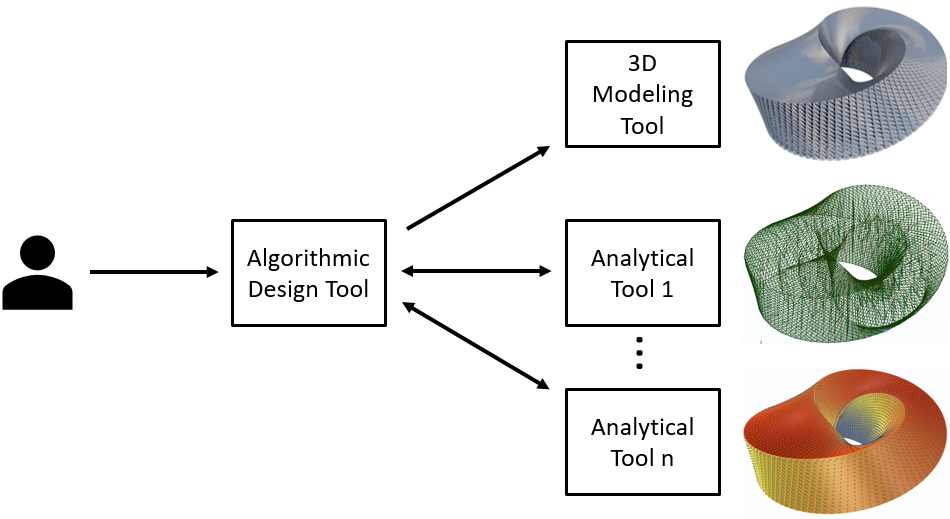
\includegraphics[width=1\textwidth]{./Images/Introduction/AlgorithmicDesignAndAnalysis_w_models2.png}
\caption[General view of the Algorithmic Design and Analysis approach]{\ac{ADA} design workflow with examples of the Astana National Library design and analytical models: (top) 3D model; (center) structural analysis model (using Robot structural analysis tool); (bottom) pos-radiation analysis model (using Radiance analysis tool).}
\label{fig:algorithmicanalysis}
\end{figure}		
	
The \ac{ADA} approach is able to enhance \ac{PBD} approaches, as it provides the means to effortlessly perform design analysis throughout the whole design process, instead of just at final stages. Depending on the performance requirements, architects might need to use different analysis tools \cite{Nguyen2014}, e.g., Daysim and Radiance for daylight analysis, EnergyPlus, TRNSYS, and DOE-2 for energy simulations, Robot Structural Analysis and Tekla Structural Designer for structural analysis.

Moreover, the \ac{ADA} approach is also important for the automation of optimization processes, as it abstracts the production of the analytical model, removing the need for direct human intervention, while reducing the occurrence of errors and information loss. Additionally, it provides the required mechanisms to quickly update a design, to generate the corresponding analytical model, to automatically evaluate the design in an analytical tool, and, finally, to collect the results and use them to guide the search for optimal solutions. 

Despite the possibility of automating optimization processes, the lack of standardized approaches is an obstacle for its application within the architectural community \cite{Attia2013}. In particular, to use such optimization processes, architects often need to acquire programming skills and invest large amounts of time and effort either to create their own optimization algorithm, to integrate dedicated optimization tools, or to include post-processing and visualization mechanisms to aid in the interpretation of the outcomes. As a result, architects rarely perform optimization or, when that is not the case, they tend to repeatedly use the same approach. While this is not always a disadvantage, it can have a negative impact in the overall optimization if, for example, architects apply inadequate algorithms over and over again.

Notwithstanding its obstacles, optimization prevailed and different approaches have spawned into the architectural practice. During this time, multiple surveys have identified the difficulties and the advantages of each approach, which enabled the development of optimization tools more targeted to architects' needs \cite{Attia2013,Nguyen2014,Shi2016}. In the following section, we briefly mention some of these approaches and we emphasize the key points of optimization processes in architecture.

% #############################################################################
\subsection{Architectural Optimization Workflow}
\label{ssec:AOW}
Recently, the emergence of \ac{AD} approaches based on visual programming, such as Grasshopper and Dynamo, together with the growing consciousness of both the benefits and limitations of optimizing building designs, led to the development of ready-to-use optimization toolsets (e.g., Galapagos and Opossum). Even though the combination of visual programming and optimization tools allowed architects to perform design optimization, architects can rarely apply it to more complex designs due to the scalability limitations generally associated with this programming paradigm \cite{Heijden2015}.

On the other hand, \ac{AD} approaches based on textual programming techniques are known to scale better with design complexity \cite{Leitao2012TPL}. In addition to the scalability benefits, its growing popularity among building design practitioners \cite{Kestelier2013}, its flexibility, and its capacity to automate optimization processes allow the development of more robust and complete optimization tools. To fully benefit from these properties, the architect must follow an optimization methodology based on the \ac{ADA} approach, where he first idealizes a design and then creates the corresponding algorithmic description, defining the parameters that represent the degrees of freedom of the design, i.e., the parameters that he is willing to manipulate. Using the design's algorithmic description, the \ac{AD} tool generates either a 3D model for visualization or analytical models for performance analysis. Optionally, the architect may decide to optimize his design according to some particular performance aspects (e.g., lighting, energy consumption, cost), potentially leading to the exploration of design solutions that were not previously considered. In that case, the optimization algorithm explores different design candidates, using the results produced by the simulation tools as the functions to optimize, returning optimal (or near optimal) design solutions.

Considering the previous view of an algorithmic-based design workflow, we identify four key aspects in an optimization process:

% ------- BEGIN \ --------
\begin{enumerate}
% ANALYTICAL MODELS
\item \textbf{Analytical models}: when the optimization algorithm specifies a candidate design, i.e., a concrete configuration for the parameters of the model, analytical models are automatically generated by the \ac{AD} tool and then used as input for the corresponding analysis tools. The level of detail and scale of an analytical model directly impacts the analysis' results and the computational time required to complete it.

% These models can be improved either through simplification of the analytical models or by enriching them with context information. The former enables the simplification of the analysis itself by providing an equivalent but simpler model to the tool, potentially reducing the simulation time, whilst the latter enables the attainment of more detailed and realistic simulations, which is not always possible due to limitations in the \ac{AD} tool. 

% OPTIMIZATION ALGORITHM
\item \textbf{Optimization algorithms}: the algorithms used to explore the design space in the quest for optimal (or near optimal) solutions. These algorithms use the results obtained in the performance analysis of different design variations as the functions to optimize, i.e., objective functions. %Generally, optimization algorithms use the inferred functions to guide the search for optimal solutions. 
The algorithm's time complexity typically depends on the number of times these functions are evaluated. In architectural design, these functions entail time-intensive simulations, which implies highly time-consuming optimization processes.

% EXPLAINABILITY / INTELLIGIBILITY OF RESULTS
\item \textbf{Intelligibility of results}: the ability to interpret and understand the design optimization results is very important within the architectural community \cite{Shi2016,Cichocka2017SURVEY}. Having access to an explanation regarding the quality of a solution allows architects to make more informed design decisions. In this way, not only can architects provide valuable arguments for the selection of a specific design solution, but they can also learn with the process, allowing them, in the future, to more quickly create designs with better performance. 

% INTERACTIVITY AND VISUALIZATION
\item \textbf{Interactivity and visualization}: interactive and visual aspects are highly important features in the context of optimization processes~\cite{Ashour2015CreativelyMOO}. On the one hand, an interactive optimization process enables the architect to use knowledge about the problem at hand, for instance, by adding or removing constraints or by exploring different, yet unexplored regions of the design space, hence potentially increasing the process' performance. On the other hand, optimization processes that provide visualizations and representations of their own evolution can present their users with better feedback about the course of the search. This feedback is important for identifying variable-objective correlations and the making of more informed design decisions about the optimization process itself, e.g., whether the evaluations made so far suffice or if the algorithm is converging to non-conventional designs that diverge from the original design intent.
\end{enumerate}

% #############################################################################
\section{Dissertation Goals}
\label{sec:goals}

This dissertation focuses on optimization problems involving expensive evaluation functions, namely, in the context of building design. Despite the evident benefits of architectural design optimization, its application within the architectural community remains infrequent. This might be explained by its considerable time complexity that goes against the time sensitiveness of most design practices~\cite{Shi2016}. Time becomes an even greater impediment when it is necessary to evaluate multiple performance aspects, instead of a single one, as it frequently happens in building design. In this case, it is of paramount importance that the optimization algorithms used are capable of efficiently handling problems involving expensive evaluation functions. Unfortunately, the currently available architectural optimization tools do not, in general, provide good algorithms for handling such problems.

This dissertation sets out to address this problem, by identifying the most adequate algorithms for optimizing computationally complex problems and exploring their application to architectural design. In this research, we consider not only building design problems involving a single performance aspect, i.e., \ac{SOO}, but also the optimization of multiple aspects simultaneously, that is, \ac{MOO}. Based on the idea that no algorithm can consistently perform better than the others on all problems~\cite{Wolpert1997NFLT}, this dissertation explores this performance difference by studying algorithms with different properties. 

The main goal of this dissertation is to identify the most efficient optimization algorithms for the different performance optimization problems that occur in building design and that frequently involve computationally heavy evaluation functions. Moreover, this dissertation aims to encapsulate these algorithms in an optimization framework that simplifies their application and, thus, promotes design optimization in architecture. To this end, the framework should include mechanisms to allow the easy specification of optimization problems, a wide variety of  algorithms to address optimization problems with different characteristics, a set of metrics that measure the quality of each algorithm, thus providing means to compare them, and informative visual representations of the obtained results.
Finally, we evaluate the proposed framework in the architectural practice and we study the behavior of different algorithms in various real \ac{BPO} problems, including the optimization of simulation-based lighting, structural, and cost aspects of designs. 

% #############################################################################
\section{Document Structure}
The following chapters are organized as follows:
\begin{itemize}
% \textbf{\Cref{chap:intro}} discusses optimization concepts and evidences its importance for different problems, ranging from simple day-to-day decisions to more complex engineering problems, such as components, circuits, and building designs. Particularly, this chapter stresses the relevance of optimization in the architectural context, providing a comprehensive overview of the existing practices and the difficulties underlying the adoption of optimization processes in architecture. \\
\item \textbf{\Cref{chap:back}} presents an overview of the current optimization practices in architecture and compares the benefits and drawbacks associated with each one.  
\item \textbf{\Cref{chap:architecture}} describes the proposed framework and enumerates important design decisions that were made during its implementation. 
\item \textbf{\Cref{chap:implement}} describes the application of the proposed framework to the architectural practice. 
\item \textbf{\Cref{chap:evaluation}} analyzes both qualitative and quantitative aspects of the proposed framework, comparing it with currently existing architectural optimization tools and evaluating multiple optimization algorithms in the context of three case studies.
\item \textbf{\Cref{chap:conclusion}} emphasizes the importance of optimization in architecture and draws some conclusions about this work and how it can influence the architectural practice. Finally, we reflect on the future improvements for the proposed framework.
\end{itemize}

% emphasizes the importance of optimization in architecture, compares the proposed framework with the currently existing architectural optimization tools, and draws some conclusions regarding the suitability of the studied algorithms. % for handling design problems that involve expensive objective functions. Moreover, it discusses the impacts of this dissertation and how it benefits the architectural practice. Finally, we reflect on the future improvements for the proposed framework. \\
